\chapter{Control architecture}
\label{chap:control}
In the course of this thesis, we divided the control of the ACTS using two separated subsystems. While the ground winches adjust the length of the lower cables to control the position of the payload relative to the ground anchors, the UAVs control the magnitude and direction of the thrust generated by their propellers to maintain the ground cables taut. 

The coordinated action of these two subsystems allows the payload to achieve the desired pose while satisfying the mechanical constraints of the system. This chapter describes the adopted control architecture and its implementation within the proposed ACTS.

\section{Force control with a point-mass payload}
Before going into details on the full consideration, let's analyze some simpler configurations.

\subsection{Case: one drone connected to the ground through a cable}
\label{sec:forceControl1droneToGround}
The goal is to design the drone force $\mathbf F_{prop}$ such as that the ground tension is controlled. Since only a tension in the cable direction is imposable, an arbitrary force $\mathbf f^*$ at the ground anchor can be achieved only by moving the drone, changing the cable direction $\mathbf u$. Called $\mathbf a$ the drone's position and $\mathbf b$ the attachment point to the ground:
\begin{equation}
    \mathbf u = \frac{\mathbf a-\mathbf b} {\|\mathbf a-\mathbf b\|}.
\end{equation}

\begin{figure}[ht]
    \centering
    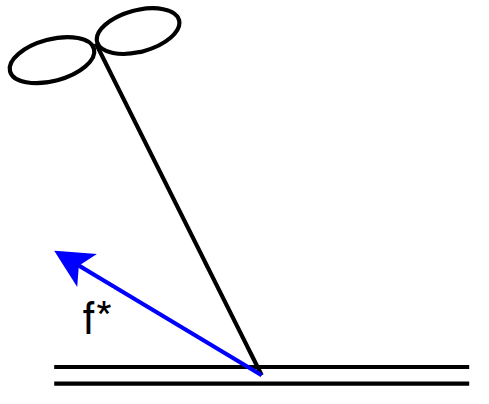
\includegraphics[width=0.3\linewidth]{images/1drone1cableGroundAnchor.png}
    \caption{One drone system connected to the ground through a cable}
    \label{fig:1drone1cableGroundAnchor}
\end{figure}

\subsubsection{Option 1}
Defined the desired cable tension $\tau^*$ and the desired cable direction $\mathbf u^*$ as:

\begin{minipage}[t]{0.45\textwidth}
\begin{equation}
    \tau^* = \|\mathbf f^*\|
    \label{eq:tau_des}
\end{equation}
\end{minipage}\hfill
\begin{minipage}[t]{0.45\textwidth}
\begin{equation} 
    \mathbf u^* = \frac{\mathbf f^*}{\|\mathbf f^*\|}
    \label{eq:u_des}
\end{equation}
\end{minipage}

\noindent The ground tension is obtained using the geometric constraint which relates the anchor point to the drone position:
\begin{equation}
    \mathbf a^* = \mathbf b + l\,\mathbf u^*
    \label{eq:geometricContraintOnUAV}
\end{equation}
where $l$ is the cable length. Equation \eqref{eq:geometricContraintOnUAV} is then used as a reference to compute the propeller force.
\begin{equation}
    \mathbf F_{\mathrm{prop}} = m_i g\,\mathbf e_3 + \mathbf K_p \left(     \mathbf a^*-\mathbf a \right) + \mathbf K_d \left(     \dot{\mathbf a}^*-\dot{\mathbf a} \right) + \tau^* \mathbf u.
\end{equation}

\subsubsection{Option 2}
Given Newton's Second Law applied to the drone described in Equation \eqref{eq:uavbalance}, we are able to estimate the cable force $\hat{\mathbf f} = \mathbf F_{a, i}^{est}$
\begin{equation}
    m_i\ddot{\mathbf a}_i = \mathbf F_{\mathrm{prop},i} - \hat{\mathbf f} + \mathbf F_{g,i} \qquad \xrightarrow{} \qquad \hat{\mathbf f} = \mathbf F_{\mathrm{prop},i} + \mathbf F_{g,i} - m_i\ddot{\mathbf a}_i
    \label{eq:uavNewton2law}
\end{equation}
where all the forces are in the world frame and $\ddot{a}_i$ is the drone linear acceleration. Using Equation \eqref{eq:uavbalance}, we would like to apply a propulsion force equal to 

\begin{equation}
    \mathbf F_{\mathrm{prop},i}^* = \mathbf f^* - \mathbf F_{g,i}.
\end{equation}
Finally, the closed loop equation is:

\begin{equation}
    \mathbf F_{\mathrm{prop},i} = \mathbf F_{\mathrm{prop},i}^* + \mathbf K_p \mathbf e + \mathbf K_d \dot{\mathbf e}, \qquad \mathbf e = \mathbf f^*-\hat{\mathbf f}.
\end{equation}
The result is given to the attitude controller, which aligns the body z-axis with the commanded thrust vector.

\subsection{Case: payload connected to the ground and a drone}
\label{sec:payload1drone1groundCable}
In this case, we are working with the simplified case of an ACTS composed by a drone, a ground anchor and a point-mass payload. Called with subscript 1 the cable that connects the payload to the drone and with 2 the one that connects it to the ground, for definition the vector $\mathbf u_i$, $i = 1\div n$ is given by 
\begin{equation}
    \mathbf u_i = \frac{\mathbf a_i-\mathbf p} {\|\mathbf a_i-\mathbf p\|}.
\end{equation}
being $\mathbf a_i$ and $\mathbf p$ respectively the actuator and the payload position.

\subsubsection{Payload position control}
The goal is to design $\mathbf F_{prop, 1}$ such that the payload reaches a desired position ($\mathbf p \xrightarrow{} \mathbf p^*$), which is reachable for the length of the cable.

\begin{figure}[h]
    \centering
    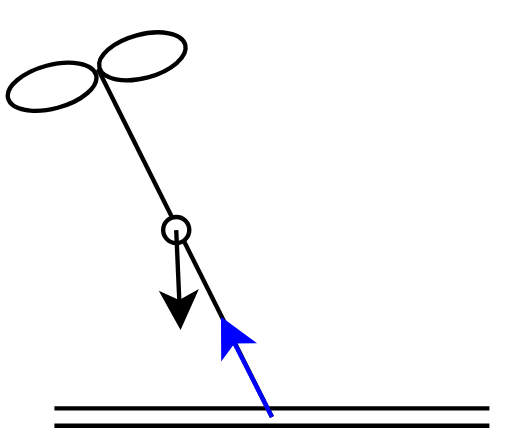
\includegraphics[width=0.3\linewidth]{images/1drone2cablesPayloadGroundAnchorTensionAlongCable.png}
    \caption{Simplified ACTS with one drone and one ground anchor}
    \label{fig:1drone2cablesPayloadGroundAnchorTensionAlongCable}
\end{figure}


The payload dynamics is given by:
\begin{equation}
\begin{aligned}
    m_p\ddot{\mathbf p} &= \tau_1\mathbf u_1 + \tau_2\mathbf u_2 - m_p g\,\mathbf e_3 \\ &= \mathbf F_{a,1} + \mathbf F_{a,2} + \mathbf F_g \\ &= \mathbf F_p + \mathbf F_g,
\end{aligned}
\qquad \xrightarrow{} \qquad
\mathbf F_p = m_p \left(\ddot{\mathbf p} + g\mathbf e_3 \right)
\label{eq:Fpdynamics}
\end{equation}

The desired payload force is defined using an impedance controller:
\begin{equation}
    \mathbf F_p^* = m_p \left(\ddot{\mathbf p}^*+g\mathbf e_3 \right) + \mathbf K_p \left(\mathbf p^*-\mathbf p \right) + \mathbf K_d \left(\dot{\mathbf p}^*-\dot{\mathbf p} \right)
    \label{eq:impedancePayloadcontrol}
\end{equation}
with $\dot{\mathbf p}^*= \mathbf 0$ and $\ddot{\mathbf p} = \mathbf 0$ as we required the payload to maintain the position once it is reached. 
The remaining force to be generated by cable 1 is:
\begin{equation}
    \mathbf F_{a,1}^* = \mathbf F_p^* - \mathbf F_{a,2},
\end{equation}
where $\mathbf F_{a,2} = \tau_2\mathbf u_2$. This brings us back to the situation in Section \ref{sec:forceControl1droneToGround}, where $\mathbf F_{a,1}$ is $\mathbf f^*$.

\subsubsection{Tension and orientation control}
The goal can also be design $\mathbf F_{prop,1}$ such that an arbitrary force $\mathbf f^*$ on the ground can be applied ($\mathbf F_2 \xrightarrow{} \mathbf f^*$). In other words, $\mathbf u_2 \xrightarrow{} \mathbf u_2^*$ and $\tau_2\xrightarrow{}\tau_2^*$. This case can be interesting to study as in a redundancy system situation, it may be helpful to add additional constraint in one of the cables.
The only difference from the previous case is that the desired position for the payload $p^*$ is not an input anymore, but obtained such that the second cable is aligned along the desired direction given by $\mathbf f^*$ (Equation \eqref{eq:tau_des} and \eqref{eq:u_des}). Then:
\begin{equation}
    \mathbf p^* = \mathbf a_2 - l_2\mathbf u_2^*.
\end{equation}

\begin{figure}[h]
    \centering
    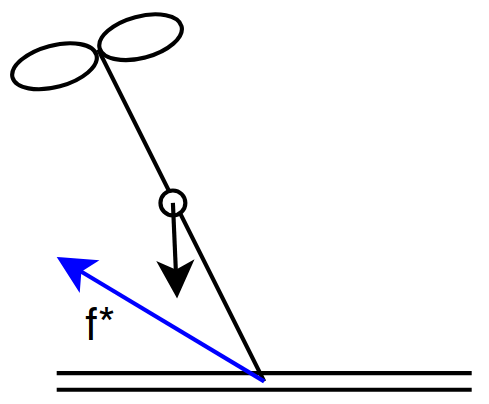
\includegraphics[width=0.25\linewidth]{images/1drone2cablesPayloadGroundAnchor.png}
    \caption{Tension directed arbitrary}
    \label{fig:1drone2cablesPayloadGroundAnchor}
\end{figure}

\subsection{Case: payload connected to the ground through two cables}
The ACTS consists of a point-mass payload connected to the ground through two cables and to a drone. The enumeration is shown in Figure \ref{fig:1drone2cablesToground}.

\begin{figure}[h]
    \centering
    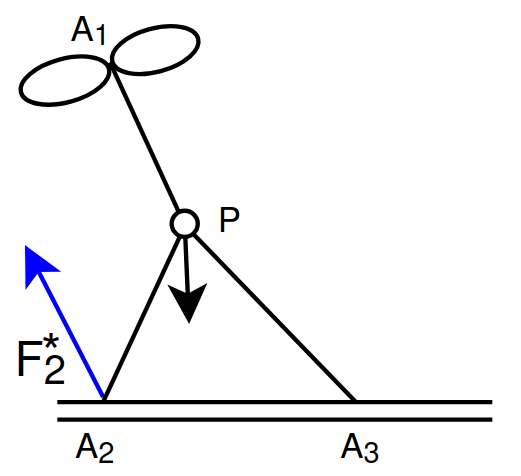
\includegraphics[width=0.3\linewidth]{images/1drone2cablesToground.png}
    \caption{Payload connected through two cable to the ground}
    \label{fig:1drone2cablesToground}
\end{figure}

\subsubsection{Payload position control}
If the input is the desired payload position $\mathbf p^*$, we find ourselves in three situations:
\begin{enumerate}
    \item $\mathbf p^*$ lies precisely on the intersecting boundary arcs dictated by the maximum lengths of the ground cables;
    \item $\mathbf p^*$ is out of reach;
    \item $\mathbf p^*$ is inside the triangle $A_1A_3P$, resulting into slack cables
\end{enumerate}

In the first case, $\mathbf p^*$ is used to compute the desired payload force $\mathbf F_p^*$ (Equation \eqref{eq:impedancePayloadcontrol}). Using the simplified payload balance equation related to the forces acting on the payload (Equation \eqref{eq:ForceOnPayload}), we obtain the following.
\begin{equation}
    \mathbf F_{a, 1}^*= \mathbf F_p^* - \sum_{i=2}^{n} \mathbf F_{a, i}
\end{equation}
which brings us back to the previous case. Because the payload is physically constrained at a boundary where both ground cables are stretched straight, any movement or external disturbance is perfectly resisted by the tension of the cables.

In the second case, since the ground cables physically block the payload from reaching $\mathbf p^*$, a steady error $\mathbf e = \mathbf p^*-\mathbf p \neq \mathbf 0$ builds up. The actual tension will be directly proportional to the control gains and the distance of the unreachable input:
\begin{equation}
    \mathbf F_{\mathrm{virtual}} \propto \left( \mathbf p^*-\mathbf p_{\mathrm{geom}} \right) \quad\implies\quad    \mathbf F_{\mathrm{virtual}} = K\left(\mathbf p^*-\mathbf p_{\mathrm{geom}}\right).
\end{equation}

where $\mathbf p_{geom}$ is the closest reachable point that lies on the workspace boundary. In this case, we may impose a controlled tension on the ground cables directed along $(\mathbf p^* - \mathbf p_{geom})$ to ensure the drone continues to pull toward the desired target:

\begin{equation}
    \mathbf F_{a,1}^* = \mathbf F_p^* - \sum_{i=2}^{n}\mathbf F_{a,i} + \mathbf F_{\mathrm{virtual}}.
\end{equation}

In the last case, the distance from the anchors to the payload is less than the cable length, resulting into slack cables as the latter cannot push. Mathematically $\tau_2= 0$ and/or $\tau_3=0$. Then, $\mathbf F_{a,1}^* = \mathbf F_p^*$.

\subsubsection{Desired tension in the cable on the ground}
The desired variable to control is the tension of one of the cables $\mathbf F_{a,2} \xrightarrow{} \mathbf f^*$. 

\begin{equation}
    \mathbf F_{a,1}^* = \mathbf F_p - \mathbf f^* - \mathbf F_{a,2},
\end{equation}
where $\mathbf F_p = m_p \left( \ddot{\mathbf p} + g\mathbf e_3 \right)$ and $ \mathbf F_{a,2} = \tau_2\mathbf u_2$.

\subsubsection{Desired tension difference between the cables on the ground}
The desired variable to control a linear combination of the two $\mathbf F_{a,2} + \alpha\mathbf F_{a,3} \xrightarrow{} \mathbf f^*$.

\begin{equation}
    \mathbf F_{a,1} = \mathbf F_p - \mathbf F_{a,2} - \mathbf F_{a,3} \qquad \implies \qquad
    \begin{aligned}
        \mathbf F_{a,1}^* &= \mathbf F_p -
        \left(
            \mathbf f^* - \alpha\mathbf F_{a,3}^* + \mathbf F_{a,3}^*
        \right) \\
        &= \mathbf F_p - \mathbf f^* - (1-\alpha)\mathbf F_{a,3}^*.
    \end{aligned}
\end{equation}
For the specific case where $ \mathbf F_{a,2} - \mathbf F_{a,3} \xrightarrow{} \mathbf f^*$:
\begin{equation}
    \mathbf F_{a,1}^* = \mathbf F_p - \mathbf f^* - 2\mathbf F_{a,3}^* = \mathbf F_p - \mathbf f^{\prime *}.
\end{equation}

\section{Extension to the complete ACTS architecture}
\label{sec:highlevelarchitecture}
At high level, the architecture that enables the system to reach the goal is shown in Figure \ref{fig:control-high-level}.
\begin{figure}[h]
    \centering
    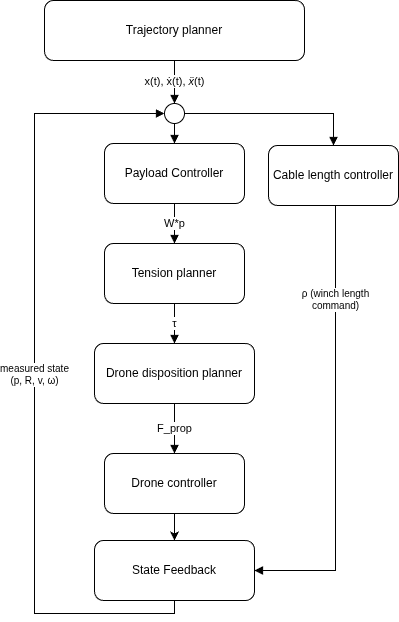
\includegraphics[width=0.61\linewidth]{images/diagrams/control_scheme.png}
    \caption{High level control scheme}
    \label{fig:control-high-level}
\end{figure}

\subsubsection{Trajectory planner}
The trajectory planner is able to compute the payload trajectory $\mathbf p(t)$ and its velocity $\dot{\mathbf p}(t)$ and acceleration $\ddot{\mathbf p}(t)$ given the system's goal, such as:
\begin{enumerate}
    \item Make the payload fly;
    \item Bring the payload at the right height and orientation;
    \item Approach the façade.
\end{enumerate}
And/or the initial and final position of the payload.

\subsubsection{Payload Controller}
Then, the desired payload wrench $W_p^*$ is computed for each point in the trajectory based on the previous state of the system. 
The desired payload wrench is computed from a geometric PD controller. The translational component is given by

\begin{equation}
    \mathbf{F}_p^* = m_p \mathbf{g} + K_p \left(     \mathbf{p}^*-\mathbf{p} \right) + K_d \left(     \dot{\mathbf{p}}^*-\dot{\mathbf{p}} \right) 
\end{equation}
where \(p^*\) and \(p\) are the desired and current payload positions, respectively. For the rotational dynamics, the controller follows the geometric formulation on \(SE(3)\) \cite{lee_geometric_2010}. The attitude error and angular velocity error are defined as
\begin{equation}
\begin{aligned}
    \mathbf{e}_R &= \frac{1}{2} \left( \mathbf{R}^{*\top}\mathbf{R} - \mathbf{R}^{\top}\mathbf{R}^* \right)^\vee \\
    \mathbf{e}_\Omega &= \boldsymbol{\Omega} - \mathbf{R}^{\top}\mathbf{R}^* \boldsymbol{\Omega}^*.
\end{aligned}
\end{equation}
Where \((\cdot)^\vee\) denotes the inverse of the skew-symmetric (hat) operator. Since the controller performs set point regulation, the desired angular velocity is zero: \(\boldsymbol{\Omega}^* = \mathbf{0}\), yielding $\mathbf{e}_\Omega = \boldsymbol{\Omega}$. The desired control moment in the world frame is then
\begin{equation}
    \mathbf{M}_p^* = \mathbf{R} \left(-K_R\mathbf{e}_R     -     K_\Omega\mathbf{e}_\Omega \right).
\end{equation}
and the desired payload wrench becomes
\begin{equation}
    \mathbf{W}_p^*
    =
    \begin{bmatrix}
        \mathbf{F}_p^* \\
        \mathbf{M}_p^*
    \end{bmatrix}.
\end{equation}

\subsubsection{Winch-Level Cable Length Controller}
When transitioning the payload to a target pose along the planned trajectory, operational priority is given to the ground actuators due to their significantly higher mechanical stiffness and positioning precision compared to UAVs.
The ground subsystem is modeled as a 6-degree-of-freedom Gough-Stewart parallel mechanism where the six ground cables act as active legs. Given the target payload position $p^*$ and target orientation matrix $\mathbf R^*$, the ideal length $\rho_i^*$ for the $i$-th ground cable is defined geometrically by:
\begin{equation}
    \rho_i^*
    =
    \left\|
        \mathbf{a}_i
        -
        \left(
            \mathbf{p}^*
            +
            \mathbf{R}^*\,{}^P\mathbf{b}_i
        \right)
    \right\|.
\end{equation}

 \begin{figure}
     \centering
     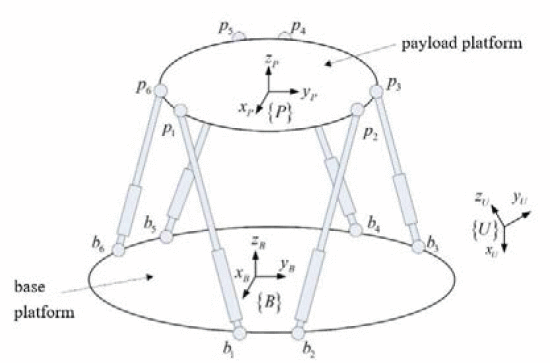
\includegraphics[width=0.5\linewidth]{images/StewartPlatform.png}
     \caption{Gough Stewart schematics \cite{wang_adaptive_2023}}
     \label{fig:stewartplatform}
 \end{figure}

To account for the finite velocity of the winch motors, the desired cable length is not applied instantaneously. Instead, the cable-length reference is updated incrementally at each control step according to

\begin{equation}
    \rho_i(t+\Delta t) = \rho_i(t) + \Delta\rho_i.
\end{equation}
where the increment $\Delta\rho_i$ is limited such that $|\Delta\rho_i| \leq v_{\max}\Delta t.$, with $v_{\max}$ being the maximum winch speed. The resulting cable-length reference is then sent to the actuator position controller. Consequently, the commanded cable length converges toward the desired value while respecting the physical velocity limits of the winch motors and avoiding unrealistically fast spool motions.

\subsubsection{Tension planner}
\label{sec:tensionPlanner}
The tension planner is the layer responsible for guaranteeing that every cable stays taut throughout the motion. In fact, when working with ACTS, a payload wrench configuration is statically admissible if and only if there exists a set of strictly positive cable tensions ($\tau_i \ge \tau_{min} > 0$) that balance the target operational wrench. This is due to the fact that cables can only pull and not push. Mathematically, this layout optimization is formulated as:

\begin{equation}
\begin{aligned}
\min_{\mathbf{p}_a} \quad
& \sum_{i=1}^{n_a} \left\| \mathbf{F}_{\mathrm{prop},i} \left(\mathbf{p}_{a,i},     \tau_{\mathrm{optimal},i} \right)
\right\|^2 + K \left\| \mathbf{J}_p^\top \boldsymbol{\tau}_{\mathrm{optimal}} - \mathbf{W}_p^* \right\|^2 \\
\text{s.t.}\quad
& x_i^2+y_i^2+z_i^2=l_i^2, \qquad \forall i\in[1,n_a] \\
& \rho_{\mathrm{WCC}}(\mathcal{U})\leq0, \\
& \rho_{\mathrm{IFC}}(\mathcal{U})\leq0.
\label{eq:tensionPlanner}
\end{aligned}
\end{equation}

Which is a Nonlinear optimization Problem (NLP) due to the Euclidean distance constraints. % In Section \ref{sec:NLPtoQP}, we propose some ways to turn it into a Quadratic Programming problem (QP).
This objective function aims to minimize the propulsion force of the drones while satisfying the wrench equilibrium equations on the payload. The parameter $K$ acts as a penalty weight that prioritizes the tracking performance over energy efficiency; setting a high value (e.g., $K=100$), heavily penalizes any mismatch between the generated wrench and the commanded target wrench $W_p^*$.

For whatever positions $p_a$, the cable tensions $\tau$ are determined by a second inner loop
\begin{equation}
\begin{aligned}
\boldsymbol{\tau}_{\mathrm{optimal}} = \underset{\boldsymbol{\tau}}{\operatorname{arg\,min}} \quad& \frac{1}{2} \boldsymbol{\tau}^{\top} \mathbf{H} \boldsymbol{\tau} \\
\text{s.t.}\quad & \mathbf{J}_p^\top(\mathbf{u}) \boldsymbol{\tau} = \mathbf{W}_p^* \\ & \tau_{\min,i} \leq \tau_i \leq \tau_{\max,i}, \qquad \forall i\in[1,n_a+n_g].
\end{aligned}
\label{eq:tension-planner}
\end{equation}
The lower bound $\tau_{min, i}>0$ in the wrench feasible condition is what enforces the taut-cable requirement.

As the winch-level control drives $\boldsymbol{\rho} \to \boldsymbol{\rho}^*$, tracking the payload's motion toward its target pose, and $\mathbf{u} \to \mathbf{u}^*$, the achievable wrench set used by the tension planner is itself changing over the trajectory, since it depends on $\mathbf{u}$. As a consequence, $\mathbf{W}_p^*$ may be reachable at the target configuration but momentarily unreachable at the actual configuration, with all tensions kept strictly positive. When this occurs, Equation \eqref{eq:tension-planner} should relax the equality constraint $\mathbf{J}_p^\top(\mathbf{u})\,\mathbf{\tau} = \mathbf{W}_p^*$ to a least-squares objective, while keeping $\tau_{min,i} > 0$ as a hard constraint. 

\begin{equation}
\begin{aligned}
\boldsymbol{\tau}_{\mathrm{optimal}} = \underset{\boldsymbol{\tau}}{\operatorname{arg\,min}} \quad& \frac{1}{2} \boldsymbol{\tau}^{\top} \mathbf{H} \boldsymbol{\tau} + \gamma \left\|     \mathbf{J}_p^\top(\mathbf{u})     \boldsymbol{\tau}     -     \mathbf{W}_p^* \right\|^2 \\ 
\text{s.t.}\quad & \tau_{\min,i} \leq \tau_i \leq \tau_{\max,i}, \qquad \forall i\in[1,n_a+n_g].
\end{aligned}
\label{eq:tension-planner-relax}
\end{equation}


This guarantees that the tension planner always returns a taut solution, one that approximates the desired wrench as closely as the actual geometry allows, rather than returning no solution at all during the transient.
For the initial stage of development, this general QP is replaced by a simplified strategy: every cable tension is fixed at the minimum admissible value,
\begin{equation}
    \tau_i^* = \tau_{\min}, \qquad \forall i\in[1,n_a+n_g].
\label{eq:tau-min-simplification}
\end{equation}



\subsubsection{Drone disposition planner}
Once the tension planner computes the scalar target tension magnitudes, the drones must dynamically adjust their orientation and propeller thrusts to impose these forces. 
From the static equilibrium balance (Equation \eqref{eq:uavbalance}) the required propeller thrust vector is given by:

\begin{equation}
\begin{aligned}
    \mathbf{F}_{\mathrm{prop},i}
    = \mathbf{F}_{a,i} - \mathbf{F}_{g,i}
    = \mathbf{J}_{a,i}^{\top}\tau_i + m_i g\mathbf{e}_3
    = T_i\,{}^0\mathbf{R}_i\,\mathbf{e}_3, \qquad T_i =
    \left\|
        \mathbf{F}_{\mathrm{prop},i}
    \right\|
\end{aligned}
\label{eq:drone-disposition}
\end{equation}
which is then handed to the attitude controller, responsible for aligning the body $z$-axis with the commanded thrust vector.

% \subsection{Quadratic Approximation of the UAV Disposition Problem}
% \label{sec:NLPtoQP}
% The nonlinear optimization problem presented in the previous section:
% $$
%     \begin{aligned}
%         \min_{p_a} \quad & \sum_{i=1}^{n_a}\|F_{prop}(p_{a, i}, \tau_{optimal})\|\\
%         \text{subj. to} \quad 
%         & x_i^2 + y_i^2 + z_i^2 = l_i^2 \quad \forall i \in [1, n_a]\\
%         & \rho_{WCC}(\mathcal{U})\le 0\\
%         & \rho_{IFC}(\mathcal{U})\le 0
%     \end{aligned}
% $$
% can be rewritten as a quadratic problem where possible.

% \subsubsection{Wrench closure condition}
% The rank condition $\text{rank}(J_p) = 6$ is not a smooth inequality. To overcome this problem, we could: 

% \begin{itemize}
%     \item Use the manipulability index squared $w^2=\det(J_p J_p^\top)\ge w_{\text{min}}^2>0$ in which $w=0$ indicates a singular configuration;
%     \item Impose positive value for the smaller singular value $\epsilon$: $\sigma_{\text{min}}(J_p) \ge \epsilon$
% \end{itemize}


% \subsubsection{The cost function}
% The objective function can be approximated by replacing the sum of Euclidean norms with the sum of squared Euclidean norms,

% \begin{equation}
%     \min_{p_a}\sum_{i=1}^{n_a}\|F_{prop}(p_{a, i}, \tau_{optimal})\| \approx \min_{p_a}\sum_{i=1}^{n_a}\|F_{prop}(p_{a, i}, \tau_{optimal})\|_2 = \min_{p_a}\sum_{i=1}^{n_a}F_{prop}^\top F_{prop}
% \end{equation}
% as for definition $\|u\|_2 = \sqrt{u^\top u}$. This approximation penalizes large outliners more than small ones.

% Therefore, the problem becomes:

% \begin{equation}
%       \begin{aligned}
%         \min_{p_a} \quad & \sum_{i=1}^{n_a}F_{prop}^\top F_{prop}\\
%         \text{subj. to} \quad 
%         & x_i^2 + y_i^2 + z_i^2 = l_i^2 \quad \forall i \in [1, n_a]\\
%         & w_{\text{min}}^2 - w^2 \le 0\\
%         & d_{\text{safe}} - d_{ij} \le 0 \\
%         & d_{\text{safe}} - d_{i} \le 0 \\
%     \end{aligned}
% \end{equation}